\chapter{Sinyal dan Sistem}

\section{Pengantar}
Sinyal dan sistem merupakan sebuah kesatuan yang saling berhubungan satu sama lain. Sinyal merupakan pola-pola bervariasi yang berubah terhadap satu atau lebih variabel bebas, yang berisi informasi tentang perilaku atau sifat dari suatu fenomena tertentu. Sistem akan menerima sinyal untuk kemudian mengelola, mengolahnya sehingga menhasilkan keluaran atau tanggapan berupa sinyal lain ataupun perilaku atau sifat tertentu sesuai keinginan. Penerapan sinyal dan sistem ada dalam banyak bidang yang bervariasi mulai dari teknologi komunikasi, elektronika, komputer, pembangkit energi, pengolahan suara untuk musik, transportasi, sampai kendali otomatis pada proses-proses di industri. Masih banyak lagi penerapan sinyal dan sistem dalam kehidupan sehari-hari yang kita sadari atau tidak telah kita gunakan secara rutin dalam kehidupan kita. Penerapan-penerapan tersebut kesemuanya memiliki pola dan ciri mendasar seperti yang telah dijabarkan pada awal paragraf. Contoh sederhananya adalah mobil. Mobil bergerak dan melaju dengan kecepatan tertentu akibat adanya injakan dari pedal gas, dalam hal ini injakan pada pedal gas merupakan sinyal masukan bagi sistem mobil dan sistem mobil melalui proses mekanis dan termodinamik pada mesinnya akan menhasilkan tanggapan berupa laju mobil yang sesuai dengan seberapa dalam injakan pedal gas. Contoh lain terdapat pada rangkaian listrik, dimana sinyal masukan berupa arus dan tegangan listrik yang berubah terhadap waktu pada sistem rangkaian listrik yang dapat berupa komponen-komponen elektronik dan elektrik seperi resistor, kapasitor dan lain-lain akan menghasilkan tanggapan berupa arus dan tegangan yang berbeda sesuai dengan yang diinginkan. 

\begin{figure}[!h]
\centering
\includegraphics[scale=0.7]{pict/sinyalsistem}
\caption{Representasi konsep sinyal dan sistem dalam diagram blok}\label{sinyalsistem}
\end{figure}

Konsep sinyal dan sistem muncul dalam dalam berbagai aplikasi yang berbeda bergantung pada bagaimana pengunaan konsep tersebut. Konsep sinyal dan sistem dapat digunakan untuk mengkaraterisasi sebuah sistem. Mengkarakterisasi berarti membaca karakter atau sifat dari sebuah sistem tertentu dengan cara memberikan sinyal masukan yang bervariasi dan membaca bagaimana sistem menanggapai masukan yang bervariasi tersebut. Hal ini seperti apabila kita mempunyai sebuah kotak hitam yang kita tidak tahu sepeti apa sifat dan bagaimana kotak hitam tersebut bekerja. Dengan memberikan masukan bervariasi terhadap kotak hitam tersebut maka akan dapat diperoleh keluaran barupa tanggapan yang berbeda dengan masukan, sehingga dengan ini kita dapat mengetahui apa dan bagaimana kotak hitam misterius ini berperilaku atau bekerja. Konsep sinyal dan sistem juga dapat digunakan untuk melakukan pemrosesan terhadap sinyal tertentu agar diperoleh keluaran sinyal sesuai yang diharapkan atau untuk menghilangkan sinyal yang tidak diinginkan. Contohnya adalah dalam sistem \textit{noise canceling} (NC) atau pembatal bising. Dalam sistem NC yang biasa digunakan pada speaker, bising atau suara mengganggu yang tidak diinginkan dari dapat diredam sedemikian hinga sehingga suara atau bunyi yang keluar dari \textit{speaker} adalah ahanya suara yang diharapkan. Sistem NC akan membangkitkan suara dengan frekuensi tertentu yang sama dengan suara bising tertentu tetapai dengan fase yang berbeda sehingga melalui proses interferensi suara bising dapat diredam. 

\begin{figure}[!h]
\centering
\includegraphics[scale=0.7]{pict/300px-Active_Noise_Reduction}
\caption{Grafik bagaimana sistem NC dapat meredam bising.  [Kredit gambar: wikimedia commons]}\label{NC}
\end{figure}
     
Penggunaan lain dari konsep sinyal dan sistem adalah pada proses kendali otomatis (\textit{automatic control system}). Sistem seperti ini digunakan untuk mengendalikan besaran-besaran fisis tertentu seperti suhu, kelembaban, ketinggian air, kecepatan aliran, arah gerak benda dan lain-lain agar besaran fisis ini berada pada nilai tertentu sesuai dengan yang diharapkan. Sistem ini umumnya tersusun atas gabungan dari beberapa sistem. Dalam sistem kendali otomatis sinyal yang diberikan oleh sensor, yang bertugas untuk merasakan suatu besaran fisis, akan digunakan oleh sistem untuk melakukan pengaturan terhadap besaran fisis seperti suhu, kecepatan laju aliran, pergerakan motor, dan lain-lain. Di dalam sistem ini sensor juga berperan sebagai pemberi umpan balik bagi sistem sehingga sistem dapat menjaga besaran fisis yang dikendalikan pada tingkat atau kuantitas yang diharapkan. Contoh dari sistem kendali otomatis ini adalah antara lain sistem \textit{autopilot} yang ada di pesawat untuk mengendalikan pesawat agar terbang pada jalur arah dan ketinggian tertentu. Contoh lain adalah sistem kendali suhu ruangan yang ada pada alat pengkondisi ruang (\textit{air conditioning}/AC), AC akan mengatur hembusan dan temperatur udara yang akan keluar dari AC sebagai tanggapan dari pembacaan sensor terhadap suhu ruangan.  

\begin{figure}[!h]
\centering
\includegraphics[scale=0.13]{pict/2000px-Feedback_Loop}
\caption{Diagram blok sistem dengan umpan balik sederhana. $X$ merupakan sinyal masukan, $Y$ merupakan sinyal tanggapan, $P_2$ adalah komponen yang memberikan umpan balik ke sistem. [Kredit gambar: wikimedia commons]}\label{umpanbalik}
\end{figure}

Untuk dapat melakukan analisis terhadap sinyal dan sistem, dibutuhkan seperangkat kerangka kerja analitis yang menggambarkan dan merepresentasikan secara matematis sinyal dan sistem tertentu yang dapat digunakan untuk memecahkan berbagai macam masalah. 
       
\section{Sinyal Waktu-Kontinu dan Sinyal Waktu-Diskrit}
Informasi dalam sebuah sinyal direpresentasikan oleh pola-pola bervariasi yang berubah terhadap variabel bebas tertentu seperti waktu. Pola-pola bervariasi yang didapatkan dari perekaman suara melalui mikrofon merupakan salah satu contoh representasi sinyal. Variasi tekanan akustik yang dirasakan oleh sensor yang ada pada mikrofon, yang sekaligus merubahnya menjadi sinyal-sinyal listrik, sebagai fungsi waktu direpresentasikan ke dalam pola-pola bervariasi tertentu. Pola-pola yang berbeda berisi informasi tentang suara-suara/kata-kata yang berbeda pula.  

\begin{figure}[!h]
\centering
\includegraphics[scale=1]{pict/speech}
\caption{Contoh sinyal hasil rekaman pembicaraan "\textit{should we chase}", tiap-tiap kata yang berbeda direpresentasikan ke dalam pola-pola bervariasi yang berbeda}\label{speech}
\end{figure} 

Secara umum sinyal dikategorikan ke dalam dua jenis yang berbeda: sinyal waktu-kontinu, dimana veriable bebasnya berubahnya secara kontinu; dan sinyal waktu-diskritm, dimana variabel bebasnya berubah hanya dalam bilangan bulat. Sinyal waktu-kontinu direpresentasikan secara matematis sebagai $x(t)$, dimana $t$ adalah variabel bebas waktu-kontinu. Sinyal waktu diskrit direpresentasikan sebagai $x[n]$, dimana $n$ merupakan variabel bebas waktu-diskrit. Sinyal hasil rekaman suara merupakan contoh sinyal waktu-kontinu. Jumlah anggaran belanja rata-rata sebagai fungsi jumlah anggota keluarga merupakan salah satu contoh dari sinyal waktu-diskrit, karena tidak mungkin jumlah anggota keluarga merupakan bilangan selain bilangan bulat seperti $1\frac{1}{2}$. Dalam pemrosesan sinyal digital, seringkali sinyal-waktu diskrit merupakan cuplikan (\textit{sampling}) dari sinyal waktu-kontinu.

\begin{figure}[!h]
\centering
\includegraphics[scale=0.9]{pict/kontinudiskrit}
\caption{(a)Sinyal waktu-kontinu $x(t)$ dan (b)sinyal waktu-diskrit $x[n]$}\label{kontinudiskrit}
\end{figure}

\section{Transformasi Sinyal}
Konsep utama dalam analisa sinyal dan sistem adalah transformasi sinyal. Transformasi sinyal juga merupakan hal yang mendasar dan penting dalam pemrosesan sinyal terutam untuk melakukan manipulasi terhadap sinyal untuk menghilangkan sinyal yang tidak diinginkan ataupun menambahkan sesuatu pada sinyal sehingga menghasilkan sinyal yang sesuai dengan yang diinginkan. 
\subsection{Contoh-contoh transformasi variabel bebas}
Ada dua macam transformasi variabel bebas yang mendasar dan penting yaitu: pergeseran waktu (\textit{time shifting}) dan penskalaan waktu (\textit{time scaling}).
\begin{enumerate}
\item \textbf{pergeseran waktu}:\\
ambil sinyal waktu-kontinu $x(t)$, sinyal ini dapat digeser dengan pengurangan oleh faktor $t_0$
\[
x'(t)=x(t-t_0).
\] 
Jika $t_0>0$, sinyal $x(t)$ akan digeser ke kanan, atau terlambat (terjadi penundaan waktu/\textit{time delay}). Sedangkan jika $t_0<0$, maka $x(t)$ akan digeser ke kiri, atau mendahului. 

\begin{figure}[!h]
\centering
\includegraphics[scale=0.9]{pict/timeshift}
\caption{Gambaran operasi pergeseran waktu [2]}\label{timeshift}
\end{figure}

Untuk kasus sinyal diskrit $x[n]$, pergeseran waktu didefinisikan sebagai
\[
x'[n]=x[n-n_0],
\]
dengan $n_0$ yang juga harus merupakan bilangan bulat. Sama halnya dengan sinyal waktu-kontinu, jika $n_0$ positif maka sinyal tergeser ke kanan dan sebaliknya jika $n_0$ negatif maka sinyal tergeser ke kiri.

\item \textbf{penskalaan waktu}:\\
Sinyal yang didapatkan dengan menskalakan variabel bebas $t$ pada sinyal kontinu didefiniskan sebagai
\begin{equation}
x'(t)=x(at).
\end{equation} 
Untuk penskalaan waktu, jika $a>1$, maka sinyal akan terkompresi atau menyusut dari sinyal $x(t)$. Jika $0<a<1$, maka sinyal akan mengembang dari sinyal $x(t)$.

\begin{figure}[!h]
\centering
\includegraphics[scale=0.7]{pict/timescaling}
\caption{Operasi penskalaan waktu pada sinyal kontinyu $x(t)$ [2]}
\end{figure}

\begin{figure}[!h]
\centering
\begin{subfigure}[b]{0.4\textwidth}
\includegraphics[width=\textwidth]{pict/timescaling1}
\caption{$x(t)=\sin \pi t$}
\end{subfigure}%
        ~ %add desired spacing between images, e. g. ~, \quad, \qquad etc.
          %(or a blank line to force the subfigure onto a new line)
\begin{subfigure}[b]{0.4\textwidth}
\includegraphics[width=\textwidth]{pict/timescaling2}
\caption{$x'_1(t)=\sin \pi 2t$}
\end{subfigure}
        ~ %add desired spacing between images, e. g. ~, \quad, \qquad etc.
          %(or a blank line to force the subfigure onto a new line)
\begin{subfigure}[b]{0.4\textwidth}
\includegraphics[width=\textwidth]{pict/timescaling3}
\caption{$x'_2(t)=\sin \pi \frac{t}{2}$}
\end{subfigure}
\caption{Efek penskalaan waktu pada sinyal sinusoidal}
\end{figure}

Untuk sinyal diskrit, penskalaan waktu didefinisikan sebagai
\begin{equation}
x'[n]=x[at]
\end{equation} 
\end{enumerate}
\subsection{Sinyal periodik}
Kelas sinyal penting yang akan sering kita jumpai dalam pemrosesan sinyal adalah sinyal periodik. Sinyal waktu-kontinu periodik $x(t)$ mempunyai sifat bahwa harga $T$-nya positif bagi
\begin{equation}
x(t) = x(t+T)
\end{equation}
untuk semua harga $t$.Sinyal periodik mempunyai sifat penting yaitu tidak berubah dengan pergeseran waktu $T$. Dalam persamaan (2.3) dikatakan bahwa $x(t)$ periodik dengan periode $T$. Jika $x(t)$ periodik dengan periode $T$, maka juga bisa dikatakan bahwa $x(t)=x(t+mT)$ untuk semua $t$ dan setiap bilangan bulat $m$. Dengan kata lain$x(t)$ juga periodik dengan periode $2T, 3T, 4T, ...$ Periode dasar $T_0$ pada $x(t)$ merupakan harga poditif terkecil $T$.

\begin{figure}[!h]
\centering
\includegraphics[scale=0.9]{pict/periodik}
\caption{Contoh sinyal periodik waktu-kontinu}
\end{figure}

Sinyal periodik pada waktu-diskrit didefinisikan sebagai
\begin{equation}
x[n]=x[n+N].
\end{equation}
Sinyal waktu diskrit $x[n]$ adalah periodik dengan periode $N$, dimana $N$ adalah bilangan bulat positif. 

\subsection{Sinyal genap dan sinyal ganjil}
Sinyal $x(n)$ atau $x[n]$ dikatakan sebagai sinyal genap jika identik terhadap waktu balikannya identik. Seperti bayangan pada cermin. Untuk sinyal waktu-kontinu didefinisikan sebagai
\begin{equation}
x(-t) = x(t),
\end{equation}
sedangkan untuk waktu-diskrit didefinisikan sebagai
\begin{equation}
x[-n]=x[n].
\end{equation}
Sinyal dikatakn sebagai sinyal ganjil jika
\begin{align}
x(-t) &= -x(t)\\
x[-n] &= -x[n].
\end{align}  
Sinyal ganjil harus 0 jika $x=0$ atau $n=0$.
\begin{figure}
\centering
\includegraphics[scale=0.9]{pict/genapganjil}
\caption{Contoh sinyal genap (a) dan ganjil (b).}
\end{figure} 

\section{Sinyal Eksponensial dan Sinyal Sinusoidal Waktu-kontinu}
Sinyal eksponensial waktu-kontinu didefinisikan dalam bentuk umum
\begin{equation}
x(t)=Ce^{at}.
\end{equation}
Ada beberapa karakteristik berbeda yang dapat ditampilkan oleh sinyal eksponensial bergantung pada parameter $C$ dan $a$ yang dilimikinya, Karakteristik-karakteristik ini ditampilkan pada tabel 2.1 berikut

\begin{table}
\centering
\caption{Beberapa karakteristik sinyal eksponensial kompleks}
\begin{tabular}{|c|c|c|}
\hline
\textbf{Karakteristik} & $C$ & $a$\\
\hline
\hline
Sinyal eksponensial real & real & real\\
\hline
Sinyal eksponensial kompleks periodik & real & imajiner\\
\hline
Sinyal eksponensial kompleks umum & kompleks & kompleks\\
\hline
\end{tabular}
\end{table}
\subsection{Sinyal eksponensial real}
Sinyal eksponensial real mempunyai komponen $C$ dan $a$ berupa bilangan real. Bergantung pada apakah nilai $a$ positif atau negatif, sinyal eksponensial real terbagi menjadi sinyal eksponensial meningkat dan sinyal eksponensial meluruh.
\[
a>0\;\;\rightarrow \text{sinyal eksponensial meningkat}
\]
\[
a<0\;\;\rightarrow \text{sinyal eksponensial meluruh}
\]
\begin{figure}[!h]
\centering
\begin{subfigure}[b]{0.4\textwidth}
\includegraphics[width=\textwidth]{pict/exponensial1}
\caption{$x_1(t)=4e^{0,5t}$}
\end{subfigure}%
\begin{subfigure}[b]{0.4\textwidth}
\includegraphics[width=\textwidth]{pict/exponensial2}
\caption{$x_2(t)=4e^{0,5t}$}
\end{subfigure}
\caption{Sinyal eksponensial meningkat (a) dan sinyal eksponensial meluruh (b)}
\end{figure}

\subsection{Sinyal eksponensial kompleks periodik}
Sinyal eksponensial kompleks periodik memiliki komponen $a$ yang imajiner. 
\begin{equation}
x(t)=e^{j\omega_0 t}
\end{equation}
Sinyal jenis ini bersifat periodik, jika kita tengok kembali persamaan (2.3) maka didapat bahwa
\[
e^{j\omega_0 t}=e^{j\omega_0 (t+T)}
\]
atau
\[
e^{j\omega_0(t+T)}=e^{j\omega_0 t} e^{j\omega_0 T}.
\]
Dari sini kita lihat bahwa suatu sinyal periodik jika 
\[
e^{j\omega_0 T} = 1.
\]
Sinyal eksponensial periodik memiliki periode dasar $T_0$,
\begin{equation}
T_0=\frac{2\pi}{|\omega_0|}.
\end{equation}
Sinyal $e^{j\omega_0 t}$ dan $e^{-j\omega_0 t}$ mempunyai periode dasar yang sama.

\subsection{Sinyal sinusoidal}
Secara umum sinyal sinusoidal didefinisikan sebagai
\begin{equation}
x(t) = A \cos (\omega_0 t + \phi),
\end{equation}
Dimana $A$ adalah amplituda sinyal, $\omega_0$ adalah frekuensi sudut dengan satuan radian per sekon, dan $\phi$ adalah fase dengan satuan radian. $\omega_0$ dapat ditulis sebagai
\[
\omega_0=2 \pi f_0,
\]
dimana $f_0$ adalah frekuensi dasar yang memiliki satuan putaran per sekon. Sinyal sinusoidal adalah sinyal periodik dengan periode dasar $T_0$. Sinyal sinusoidal memiliki hubungan dengan sinyal eksponensial periodik melalui hubungan Euler
\begin{equation}
e^{j\omega_0 t}=\cos \omega_0 t + j \sin \omega_0 t.
\end{equation}
Kita bisa mengekspresikan sinyal sinusoidal ke dalam komponen real dan imajiner eksponensial kompleksnya.
\begin{align}
A\cos (\omega_0 t+\phi)&=A \Re\lbrace e^{(j\omega_0t+\phi)}\rbrace\\
A\sin (\omega_0 t +\phi)&= A\Im\lbrace e^{(j\omega_0 t+\phi)}\rbrace. 
\end{align}
Selain itu, sinyal sinusoidal juga dapat dituliskan ke dalam sinyal eksponensial periodik melalui
\begin{equation}
A\cos (\omega_0 t+\phi)=\frac{A}{2}e^{j\phi}e^{j\omega_0 t} + \frac{A}{2} e^{-j \phi} e^{-j\omega_0 t}. 
\end{equation} 

\begin{figure}
\centering
\includegraphics[scale=0.4]{pict/sinusoidal}
\caption{Contoh sinyal sinusoidal $x(t)=2\cos (2\pi t+\frac{\pi}{6})$}
\end{figure}

\subsection{Sinyal eksponensial kompleks umum}
Sinyal eksponensial kompleks umum memilik komponen $C$ dan $a$ berupa bilangan kompleks. Dalam hal ini $C$ diekspresikan ke dalam bentuk polar ($re^{j \phi}$), sedangkan $a$ ke dalam bentuk rektangular ($x+jy$). 
\begin{align*}
C&=|C|e^{j\phi}\\
a&=r+j\omega_0.
\end{align*}
Maka sinyal eksponensial kompleks umum dituliskan sebagai
\begin{equation}
Ce^{at}=|C|e^{j\phi}e^{(r+j\omega_0)}=|C|e^{rt}e^{j(\omega_0 t+\phi)}.
\end{equation}
Dengan menggunakan hubungan Euler, kita dapat memperluasnya menjadi
\begin{equation}
Ce^{at}=|C|e^{rt} \cos(\omega_0 t+\phi)+j|C|e^{rt}\sin(\omega_0 t+\phi).
\end{equation}
Untuk nilai $r$, jika
\begin{align*}
r=0\;\;&\rightarrow \text{bagian real dan imajiner eksponensial kompleks adalah sinusoidal}\\
r>0\;\;&\rightarrow \text{sinyal sinusoidal meningkat}\\
r<0\;\;&\rightarrow \text{sinyal sinusoidal meluruh atau teredam}
\end{align*}

\begin{figure}[!h]
\centering
\begin{subfigure}[b]{0.5\textwidth}
\includegraphics[width=\textwidth]{pict/sinusturun}
\caption{$x_1(t)=4e^{-0,5t}\cos(2\pi t)$}
\end{subfigure}%
\begin{subfigure}[b]{0.5\textwidth}
\includegraphics[width=\textwidth]{pict/sinusnaik}
\caption{$x_2(t)=4e^{0,5t}\cos(2\pi t)$}
\end{subfigure}
\caption{Sinyal sinusoidal meningkat (a) dan sinyal sinusoidal meluruh atau teredam (b).}
\end{figure}

\section{Sinyal Eksponensial Kompleks dan Sinyal Sinusoidal Kompleks Waktu-Diskrit}
